\documentclass[,man,floatsintext]{apa6}
\usepackage{lmodern}
\usepackage{amssymb,amsmath}
\usepackage{ifxetex,ifluatex}
\usepackage{fixltx2e} % provides \textsubscript
\ifnum 0\ifxetex 1\fi\ifluatex 1\fi=0 % if pdftex
  \usepackage[T1]{fontenc}
  \usepackage[utf8]{inputenc}
\else % if luatex or xelatex
  \ifxetex
    \usepackage{mathspec}
  \else
    \usepackage{fontspec}
  \fi
  \defaultfontfeatures{Ligatures=TeX,Scale=MatchLowercase}
\fi
% use upquote if available, for straight quotes in verbatim environments
\IfFileExists{upquote.sty}{\usepackage{upquote}}{}
% use microtype if available
\IfFileExists{microtype.sty}{%
\usepackage{microtype}
\UseMicrotypeSet[protrusion]{basicmath} % disable protrusion for tt fonts
}{}
\usepackage{hyperref}
\hypersetup{unicode=true,
            pdftitle={Early language experience in a Papuan village},
            pdfauthor={Marisa Casillas, Penelope Brown, \& Stephen C. Levinson},
            pdfkeywords={Child-directed speech, linguistic input, non-WEIRD, vocal maturity, turn
taking, interaction, Papuan},
            pdfborder={0 0 0},
            breaklinks=true}
\urlstyle{same}  % don't use monospace font for urls
\usepackage{graphicx}
% grffile has become a legacy package: https://ctan.org/pkg/grffile
\IfFileExists{grffile.sty}{%
\usepackage{grffile}
}{}
\makeatletter
\def\maxwidth{\ifdim\Gin@nat@width>\linewidth\linewidth\else\Gin@nat@width\fi}
\def\maxheight{\ifdim\Gin@nat@height>\textheight\textheight\else\Gin@nat@height\fi}
\makeatother
% Scale images if necessary, so that they will not overflow the page
% margins by default, and it is still possible to overwrite the defaults
% using explicit options in \includegraphics[width, height, ...]{}
\setkeys{Gin}{width=\maxwidth,height=\maxheight,keepaspectratio}
\IfFileExists{parskip.sty}{%
\usepackage{parskip}
}{% else
\setlength{\parindent}{0pt}
\setlength{\parskip}{6pt plus 2pt minus 1pt}
}
\setlength{\emergencystretch}{3em}  % prevent overfull lines
\providecommand{\tightlist}{%
  \setlength{\itemsep}{0pt}\setlength{\parskip}{0pt}}
\setcounter{secnumdepth}{0}
% Redefines (sub)paragraphs to behave more like sections
\ifx\paragraph\undefined\else
\let\oldparagraph\paragraph
\renewcommand{\paragraph}[1]{\oldparagraph{#1}\mbox{}}
\fi
\ifx\subparagraph\undefined\else
\let\oldsubparagraph\subparagraph
\renewcommand{\subparagraph}[1]{\oldsubparagraph{#1}\mbox{}}
\fi

%%% Use protect on footnotes to avoid problems with footnotes in titles
\let\rmarkdownfootnote\footnote%
\def\footnote{\protect\rmarkdownfootnote}


  \title{Early language experience in a Papuan village}
    \author{Marisa Casillas\textsuperscript{1}, Penelope Brown\textsuperscript{1},
\& Stephen C. Levinson\textsuperscript{1}}
    \date{}
  
\shorttitle{Early language experience in a Papuan village}
\affiliation{
\vspace{0.5cm}
\textsuperscript{1} Max Planck Institute for Psycholinguistics}
\keywords{Child-directed speech, linguistic input, non-WEIRD, vocal maturity, turn taking, interaction, Papuan\newline\indent Word count: XXXXX (XXXX not including references)}
\usepackage{csquotes}
\usepackage{upgreek}
\captionsetup{font=singlespacing,justification=justified}

\usepackage{longtable}
\usepackage{lscape}
\usepackage{multirow}
\usepackage{tabularx}
\usepackage[flushleft]{threeparttable}
\usepackage{threeparttablex}

\newenvironment{lltable}{\begin{landscape}\begin{center}\begin{ThreePartTable}}{\end{ThreePartTable}\end{center}\end{landscape}}

\makeatletter
\newcommand\LastLTentrywidth{1em}
\newlength\longtablewidth
\setlength{\longtablewidth}{1in}
\newcommand{\getlongtablewidth}{\begingroup \ifcsname LT@\roman{LT@tables}\endcsname \global\longtablewidth=0pt \renewcommand{\LT@entry}[2]{\global\advance\longtablewidth by ##2\relax\gdef\LastLTentrywidth{##2}}\@nameuse{LT@\roman{LT@tables}} \fi \endgroup}


\usepackage{lineno}

\linenumbers

\authornote{

Correspondence concerning this article should be addressed to Marisa
Casillas, P.O. Box 310, 6500 AH Nijmegen, The Netherlands. E-mail:
\href{mailto:Marisa.Casillas@mpi.nl}{\nolinkurl{Marisa.Casillas@mpi.nl}}}

\abstract{
To be completed later.


}

\begin{document}
\maketitle

\section{Introduction}\label{intro}

In their first five years of life, children hear an extraordinary amount
of language in a wide variety of interactional contexts. Tracking the
distribution and characteristics of this linguistic input over the day,
across age, and between children is a difficult task. Until recently,
developmental language science has relied on short video recordings of
caregiver-child interaction, at home or in the lab, to get a grasp on
what kinds of language children typically hear. This has been a fruitful
approach in teasing out individual and group-based differences in
interactional style (REFS). However, short recordings are limited in
their insight because they represent only a small slice of the child's
language abilities and experiences (REFS).

Improved recording hardware and advances in speech technology have
recently allowed us to use daylong recordings to get a peek into
children's broader language landscapes. Daylong recordings are made with
a device, usually positioned on the target child's chest, while that
child freely navigates their social environment for most of a waking day
(REFS). This style of audio recording has allowed researchers to track
children's verbal language use across a range of activity and
interlocutor contexts, yielding more representative and generalizable
measures of their language environments (REFS). While daylong recording
collections are typically too large for comprehensive transcription and
annotation, a combination of automated tools, (REFS) sampling techniques
(REFS), and standardized annotation approaches (REFS) can lead to rich,
but efficiently-gained glimpses into the at-home language environment.
However, properly collecting, processing, and archiving daylong data is
not easily achieved and may not be well suited for a range of research
questions (REFS). At time of writing, there are few options for
capturing visual information across the day (but see REFS), limiting
this method primarily to acoustic phenomena (REFS).

Daylong recording methods are still relatively new, and their
reliability and predictive value for language development have not yet
been fully established. For example, one collection of recordings made
in the US Northwest suggests that there is so much variability across
activities and days in basic talk characteristics (e.g., how much speech
comes from what types of speakers) that researchers need several days of
recordings before they can expect their input estimates to stabilize
(Anderson \& Fausey, in prep). Even if one can achieve a reliable
estimate of a language environment measure (e.g., overhearable adult
words per hour), how and why that estimate relates to deeper factors
shaping the learning situation, including caregiving ideologies and
language outcomes, is often indirect at best. Relatedly, meaningful
differences between individual children may be minimized when averaging
across the entirety of the day's high and low moments; it may well be
that a few key interactions throughout the day provide sharper
resolution on individual and group-based differences compared to
whole-day averages.

Two recent studies have directly investigated the effect of recording
duration on caregiver speech, finding that short recordings display
denser, somewhat different input than what is found in longer recordings
(REFS). Bergelson and colleagues (REFS) analyzed the contexts of noun
use encountered by 44 6- and 7-month-old children in the US in both
hour-long at-home videos and daylong recordings. The hour-long video
differed from the day-long average in the density of noun input, the
utterances in which nouns were embedded (e.g., questions
vs.~declaratives), and the actual nouns used. When the authors compared
the hour-long video to the \enquote{peak} hour of talk in the day, they
found a similar density of noun input across the recording types, but
the other differences remained. This difference in input density also
appears in short recordings of varying length with US children (REFS).
Importantly, however, the speech characteristics heard by individual
children in a sample correlates across recording types (i.e., their
relative rank for a given measure is stable; REFS). Based on these
findings, one could infer that at-home short recordings are influenced
by some (but not all) of the same underlying factors that drive language
patterns during daylong recordings (e.g., caregiver ideologies about
child development, child responsiveness, household composition).

Studies of children growing up in two indigenous Mayan communities of
Southern Mexico (Tseltal and Yucatec Mayan) suggest that short and long
recordings may yield substantial differences in how the speech
environment is characterized (REFS). Previous studies on these
communities have tended to use ethnographic and microanalytic analyses
of short interactions to examine the character of children's speech
environments. They have found that caregivers shape infants' and young
children's worlds such that the children learn to attend to what is
going on around them rather than expecting to be the center of attention
(REFS). Consistent with this goal, direct talk to infants, particularly
from adults, is rare until children themselves begin to elicit responses
from others (REFS). Because young children are often cared for by older
siblings and cousins, a substantial portion of talk to young children
was also expected to come from other children (REFS). Similar
observations have been reported for multiple other distinct (but
ethnolinguistically related) communities in the region (REFS). Following
up on this ethnographic work, Shneidman (REFS) used short videos of
interaction to conduct a quantitative, longitudinal study of the speech
young Yucatec children heard. She found that interactional patterns
aligned well with observations in previous work in that community:
infants were rarely spoken to at first, but their language input
increased enormously with age, mostly due to an influx of speech from
other children (REFS). However, when Casillas and colleagues (REFS) used
daylong recordings with a Tseltal Mayan community, where a similar
caregiver interactional style has been described previously on the basis
of short videos, the pattern of findings diverged from expectations. In
brief, they found that infants and young children were indeed spoken to
rarely, but that there was no increase in speech input with age and the
majority of speech came from adult women, even when children were old
enough to independently follow their older siblings and cousins around
the house. These divergent results betweeh daylong and short video
recordings don't imply that the latter is wrong, only that it is not
representative with respect to the child's language experience over an
entire day.

These findings do raise an important issue faced by developmental
psychology as it continues to expand the study of child language to more
diverse speech communities: when researchers are not members of the
community they are studying, it is difficult to know a priori what is
typical, representative, or meaningful in children's language
experience. By observing as much speech as possible in a context as
ecologically valid as possible and by sampling, annotating, and
analyzing the data on the basis of the most established development
measures we have, researchers using daylong recordings might hope to
approach this issue without first needing to conduct deep ethnographic
studies in the community on caregiving practices and ideologies around
language use and language development (REFS). When studying members of
our own cultural group, we can bridge between simple, observable
behaviors and rich interpretations of, thereby expanding our explanatory
model beyond the measures directly analyzed (e.g., why child-directed
talk might relate to faster vocabulary development). We cannot hope to
gain such enriched understandings cross-culturally without ethnographic
work; and in the absence of such work we must accept that there may be a
dissociation between how we have traditionally understood an
operationalized language behavior (e.g., child-directed speech) and what
drives the use and form of that behavior in a given community or
interactional context (e.g., pedagogical concerns, entertainment of the
caregiver, getting the child to assist). Until there are trained
researchers working on this topic who were born and raised as members of
these communities (what we should be trying to cultivate for the longer
term) this is a quandary we will continue to face.

Pairing ethnographic work with broader-scope studies of children's
language environments may be the most fruitful way to ensure that their
speech environments and speech development are captured well enough to
propose and test meaningful theories cross-culturally. These two methods
have complementary roles to play in exploring the landscape of at-home
language, and neither should be taken to reflect the \enquote{true}
language input for a given child; after all, in the example of Tseltal
above, many interactions with infants during the daylong recordings came
during moments where visitors using a video camera, or even other
community members, would not typically be invited (e.g., after the
parent was roused by the child, who was waking from an afternoon sleep).
If we want to encourage more work on small-scale and/or understudied
language learning contexts, it will be important to continue
establishing how different methods of measuring the input impact the
conclusions that are likely to be made.

In this study we present analyses of daylong recordings from a
small-scale indigenous community in which prior ethnographic work has
painted a clear picture of early caregiver-child interaction, different
from what we have seen in studies of Mayan caregivers: child-centric,
face-to-face interaction from the first days of infancy on Rossel
Island, Papua New Guinea (PNG). In what follows we will review the
ethnographic work done with this community previously, our methods for
following up on these findings with daylong recordings, and a discussion
of the differences that arose. This study was completed as part of a
larger comparative project focusing on children's speech environments
and linguistic development at two sites: the Tseltal Mayan community
mentioned above (Casillas et al., forthcoming) and this Rossel Island
community. Therefore all methods for annotation and analysis in this
study parallel those reported elsewhere for Tseltal Mayan children's
speech environments (Casillas, Brown, \& Levinson, forthcoming).

\subsection{The community}\label{the-community}

Yélî Dnye is a language spoken by approximately 5000 people, nearly all
of whom reside on Rossel Island, a remote island 250 nautical miles off
the mainland coast in Milne Bay Province, Papua New Guinea. While all
the neighboring languages fall into the Austronesian family, Rossel is a
presumed-Papuan isolate that features a phonological inventory and set
of grammatical features that are completely unattested in other
languages of the region. Partly due to its remoteness, most children on
Rossel Island grow up speaking it monolingually at home, only beginning
to learn English (the official lingua franca of Milne Bay Province) as
they progress through school, which typically begins when a child is 7
or 8 years old.

We were interested to investigate the language environment of children
acquiring Yélî Dnye because prior ethnographic work had suggested that
child-directed speech is highly frequent in this community, from mothers
and other adult caregivers, but also from other children. Therefore we
were interested in understanding how children's input environment
influenced their acquisition of this language with all its rare
structures.

However, to our surprise we found that Yélî children were not spoken to
very often at all. In fact, they were spoken to less often than the
Tseltal children we have studied in other work, who are growing up in a
community where children are indeed reportedly spoken to infrequently.

\subsection{Our predictions}\label{our-predictions}

Based on prior ethnographic work, we expected to see that young children
and infants are spoken to relatively frequently---on par with Western
children, and certainly more often than we saw with Tseltal children,
where estabished work from a number of related ethnolinguistic groups
suggests a non-child-centric approach to early language socialization.
Because of the similar subsistence farming lifestyle we expected that,
like Tseltales, Rossel Island children would show strong time-of-day
effects. Similarly, because children in both sites are growing up in
large households, we expected to see lots of ODS and, consistent with
both Tseltal and NA data, a decrease in ODS with age. We predicted an
increasing proportion of speech from other children in Tseltal but
didn't find it; ethnographic predictions on Rossel would say the
same\ldots{} so we expect it again. Do we expect an increase in CDS with
age??

\section{Method}\label{method}

This study was completed as part of a larger comparative project
focusing on children's speech environments and linguistic development at
two sites: a Tseltal Mayan community in southern Mexico and this Rossel
Island community. Therefore all methods for annotation and analysis in
this study parallel those reported elsewhere for Tseltal Mayan
children's speech environments (Casillas, Brown, \& Levinson,
forthcoming).

The data we present come from 7--9-hour recordings of a waking day at
home for the child. Children wore the recording device, which was an
elastic vest containing a small stereo audio recorder (Olympus WS-832 or
WS-853) and a miniature camera that captured photos of the child's
frontal view at a fixed interval (every 15 seconds; Narrative Clip 1).
The camera was additionally outfitted with a fisheye lens that, while
distorting the images, allowed us to capture 180 degrees of children's
frontal view. Because the camera and recorder are separate devices, they
were synchronized using an external wristwatch that was used to record
the current time at start of recording on each device individually, with
accuracy down to the second (photographed by the camera and spoken into
the recorder). The photos are timestamped by the camera such that the
precise intervals between photos are captured. These timestamps can be
used with the cross-device time synchronization cue to create
photo-linked audio files of each recording, which we then format as
video files (see REFS-URL for scripts and more information).

We chose to collect multi-hour recordings of children's language
experience at home in order to capture a range of different activity
contexts and interlocutors at different times of day (REFS). Previous
work investigating the trade-offs of short- versus long-format
recordings of parental speech have demonstrated that the apparent
quantity of speech children hear and some of the characteristics of that
speech differs depending on recording duration (day-by-day tamislemonda
REFS). That said, short recordings often have the benefit of video data,
which enables analysts to take visual information into account in
interpreting the communicative behaviors captured. Those using daylong
recording methods instead have traditionally had to sacrifice this
visual context because of (current) technological limitations; there are
no miniature, lightweight (e.g., 400g; 5cm x 5cm or less) video
recorders on the market that can record for 7--16 hours. We aimed to
generate generalizable baseline estimates of how much speech children
hear in this community but wanted to maintain visual information for
later transcription and interpretation, leading to us develop this novel
daylong recording method (see also Abels REFS).

This set-up was used to create daylong recordings of 57 children under
age 4;0 on Rossel Island in 2016 (Casillas et al HB), from which we
selected 10 representative children between ages 0;0 and 3;0 for
transcription and analysis in the current study. The 10 children were
selected to be spread between the target age range (0;0--3;0) while also
representing a range of typical maternal education levels found in the
community and being evenly split between male and female children (see
also ACLEW REFS). For each child we then selected a series of
non-overalapping sub-clips from the day for transription in the
following order: nine randomly-selected 2.5-minute clips, five
manually-selected \enquote{peak} turn-taking activity 1-minute clips,
five manually-selected \enquote{peak} vocal activity 1-minute clips, and
one manually-selected 5-minute expansion of the best one-minute clip,
for a total of 37.5 minutes of transcribed audio for each child (6.25
audio hours in total). The criteria for manual clip selection are
identical to those described for the parallel study on Tseltal by
Casillas and colleagues (forthcoming).

We were limited to selecting sub-clips from 10 children for analysis
because of the time-intensive nature of transcribing these naturalistic
data; 1 minute of audio typically took us approximately 60--70 minutes
to be segmented into utterances, transcribed, annotated, and loosely
translated into English (\textasciitilde{}400 hours total). Given that
Yélî Dnye is nearly exclusively spoken on Rossel Island, where there is
no electricity and unreliable access to mobile data, transcription could
only be completed over the course of three 4--6 week visits by our
research group to the island in 2016, 2018, and 2019.

We used the ACLEW Annotation Scheme (REFS) in ELAN (ELAN REFS) to
transcribe and annotate all hearable speech---both near and distant---in
the clips. We first segmented out the utterances and ascribed them to
individual speakers (e.g., older brother, mother, aunt, etc.). We then
annotated the vocal maturity of each utterance produced by the target
child (non-canonical babble/canonical babble/single
word/multi-word/unsure) and annotated the addressee of all speech from
other speakers (addressed to the target child/one or more other
children/one or more adults/a mix of adults and children/any
animal/other/unsure). Transcription and annotation was done together by
the first author and one of three community members (all native speakers
of Yélî Dnye). The community-based research assistants personally knew
all the families in the recordings, and were able to use their own
experience, the discourse context, and information from the accompanying
photos in reporting what was said and to whom speech was addressed for
each utterance. Detailed manuals and self-guided training materials,
including a \enquote{gold standard test} for this annotation scheme can
be found at URL (REFS).

\begin{table}[tbp]
\begin{center}
\begin{threeparttable}
\caption{\label{tab:tab1}Demographic overview of the 10 children whose recordings are sampled in the current study, including from left to right: child's age (years;months.days); child's sex (M/F); mother's age (years); level of maternal education (none/primary/secondary/preparatory/university); and the number of people living in the child's household.}
\begin{tabular}{lllll}
\toprule
Age & \multicolumn{1}{c}{Sex} & \multicolumn{1}{c}{Mother's age} & \multicolumn{1}{c}{Level of maternal education} & \multicolumn{1}{c}{People in household}\\
\midrule
01m;09d & F & 31 & secondary & 8\\
16m;29d & M & 25 & secondary & 6\\
20m;03d & F & 33 & primary & 9\\
35m;29d & M & 41 & primary & 8\\
12m;29d & F & 30 & primary & 9\\
04m;13d & M & 24 & preparatory & 5\\
25m;22d & F & 21 & secondary & 4\\
03m;19d & M & 37 & primary & 9\\
09m;03d & F & 29 & secondary & 5\\
07m;18d & M & 24 & secondary & 5\\
\bottomrule
\end{tabular}
\end{threeparttable}
\end{center}
\end{table}

\begin{figure}
\centering
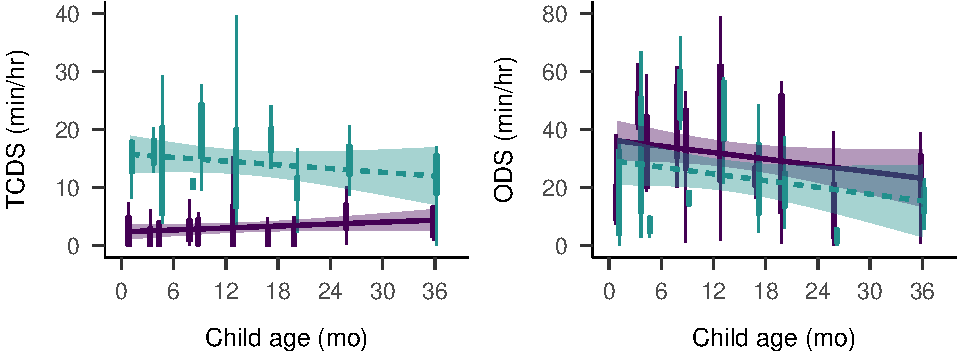
\includegraphics{Yeli-CLE_files/figure-latex/fig2-1.pdf}
\caption{\label{fig:fig2}Recording duration (black line) and sampled clips
(colored boxes) for each of the 10 recordings analyzed, sorted by child
age in months.}
\end{figure}

\begin{verbatim}
## pdf 
##   2
\end{verbatim}

\begin{verbatim}
## pdf 
##   2
\end{verbatim}

\begin{verbatim}
## pdf 
##   2
\end{verbatim}

\begin{verbatim}
## pdf 
##   2
\end{verbatim}

\begin{figure}
\centering
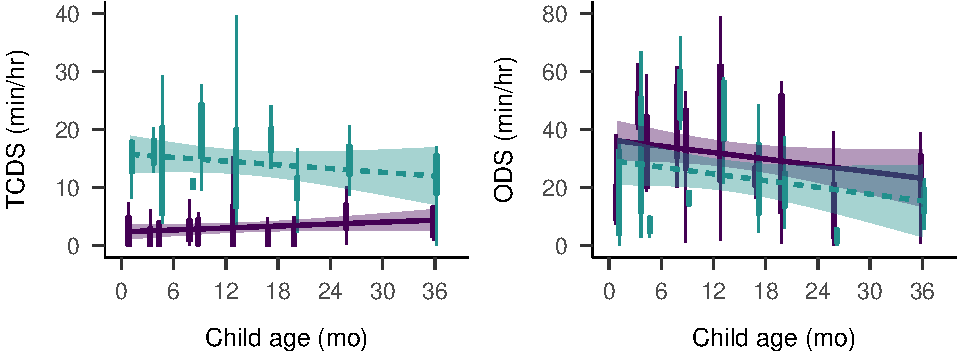
\includegraphics{Yeli-CLE_files/figure-latex/fig3-1.pdf}
\caption{\label{fig:fig3}Estimates of TCDS min/hr (left) and ODS min/hr
(right) across the sampled age range. Each box plot summarizes the data
for one child from the randomly sampled clips (purple; solid) or the
turn taking clips (green; dashed). Bands on the linear trends show 95\%
confidence intervals.}
\end{figure}

\begin{figure}
\centering
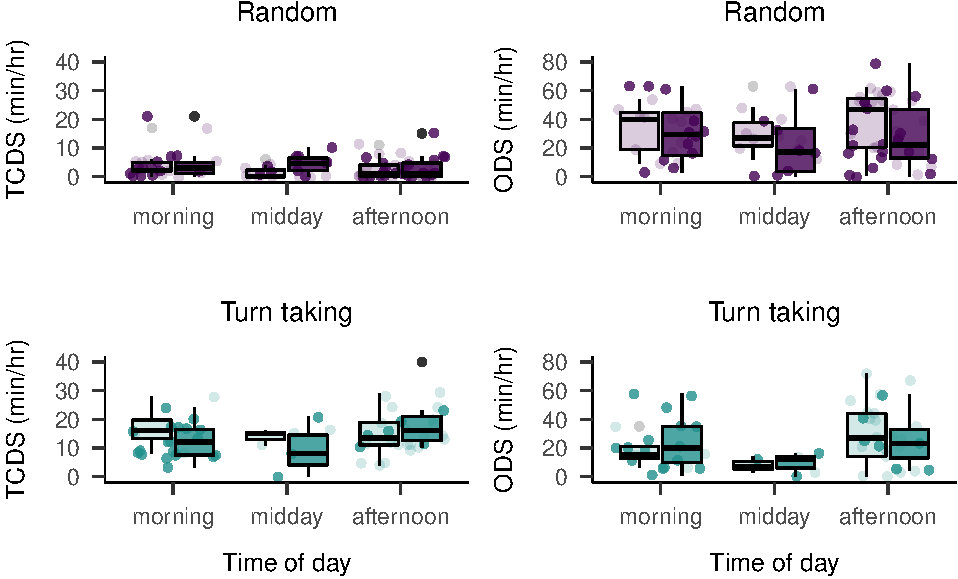
\includegraphics{Yeli-CLE_files/figure-latex/fig5-1.pdf}
\caption{\label{fig:fig5}Estimates of TCDS min/hr (left panels) and ODS
min/hr (right panels) across the recorded day in the random clips (top
panels) and turn-taking (bottom panels) clips. Each box plot summarizes
the data for children age 1;0 and younger (light) or age 1;0 and older
(dark) at the given time of day.}
\end{figure}

\begin{verbatim}
## [1] 3.13
\end{verbatim}

\begin{verbatim}
## [1] 2.95
\end{verbatim}

\begin{verbatim}
## [1] 1.58
\end{verbatim}

\begin{verbatim}
## [1] 6.26
\end{verbatim}

\begin{verbatim}
## [1] 14.49
\end{verbatim}

\begin{verbatim}
## [1] 15.07
\end{verbatim}

\begin{verbatim}
## [1] 9.54
\end{verbatim}

\begin{verbatim}
## [1] 18.73
\end{verbatim}

\begin{verbatim}
## [1] 73.32
\end{verbatim}

\begin{verbatim}
## [1] 78.84
\end{verbatim}

\begin{verbatim}
## [1] 41.41
\end{verbatim}

\begin{verbatim}
## [1] 100
\end{verbatim}

\begin{verbatim}
## [1] 35.9
\end{verbatim}

\begin{verbatim}
## [1] 32.37
\end{verbatim}

\begin{verbatim}
## [1] 20.2
\end{verbatim}

\begin{verbatim}
## [1] 53.78
\end{verbatim}

\begin{verbatim}
## [1] 28.81
\end{verbatim}

\begin{verbatim}
## [1] 21.22
\end{verbatim}

\begin{verbatim}
## [1] 6.68
\end{verbatim}

\begin{verbatim}
## [1] 60.18
\end{verbatim}

\subsection{Vocal maturity}\label{vocal-maturity}

\begin{verbatim}
## pdf 
##   2
\end{verbatim}

\begin{verbatim}
## pdf 
##   2
\end{verbatim}

\begin{verbatim}
## pdf 
##   2
\end{verbatim}

\begin{figure}
\centering
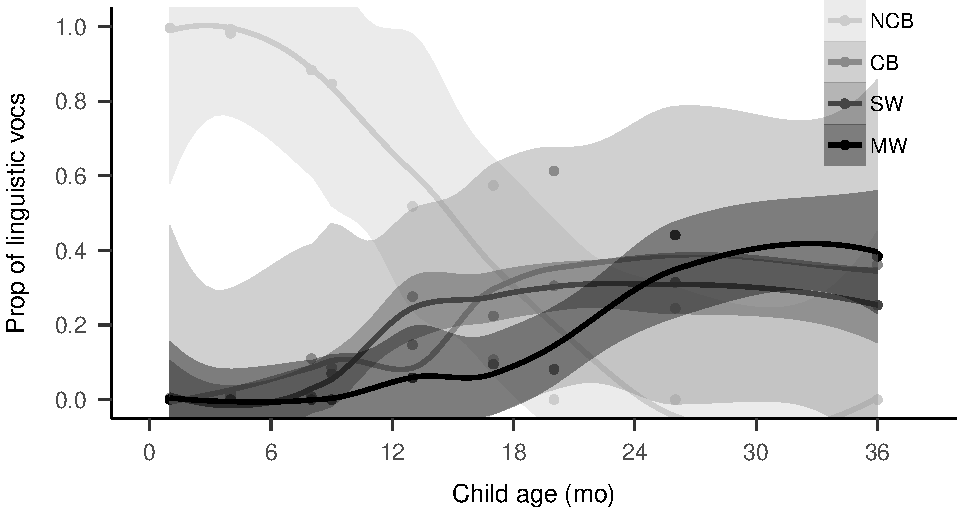
\includegraphics{Yeli-CLE_files/figure-latex/fig6-1.pdf}
\caption{\label{fig:fig6}Proportion of vocalization types used by children
across age (NCB = Non-canonical babble, CB = Canonical babble, SW =
single word utterance, MW = multi-word utterance).}
\end{figure}

\section{Acknowledgements}\label{acknowledgements}

This paper was written using the papaja library in RStudio (Aust \&
Barth, 2018).

\newpage

\section{References}\label{refs}

\begingroup
\setlength{\parindent}{-0.5in} \setlength{\leftskip}{0.5in}

\hypertarget{refs}{}
\hypertarget{ref-R-papaja}{}
Aust, F., \& Barth, M. (2018). \emph{papaja: Create APA manuscripts with
R Markdown}. Retrieved from \url{https://github.com/crsh/papaja}

\endgroup


\end{document}
